\section{消失黏性}
\label{sec:hj-vanishing}

第~\ref{chap:pde-problems}章已经见过，给程函方程加一个小扩散项，解的极限就是到边界的距离。这一节解释这个现象：在方程中加入$\varepsilon\Delta u$，光滑解在$\varepsilon\to0$时为什么收敛到黏性解，以及有限的$\varepsilon$下误差有多大。

考虑带小扩散的方程
\begin{equation}
  \partial_tu_\varepsilon+H(\nabla u_\varepsilon)=\varepsilon\Delta u_\varepsilon,\qquad u_\varepsilon(\cdot,0)=u_0,
  \label{eq:hj-viscous}
\end{equation}
其中$\varepsilon>0$。$\varepsilon$前面的符号与第~\ref{chap:diffusion-equations}章的热方程相同，时间向前是适定的。

\paragraph{一个可以精确求解的例子}
对$H=\lVert\bm{p}\rVert_2^2/2$，式~\eqref{eq:hj-viscous}可以化成线性的热方程。设$u_\varepsilon=-2\varepsilon\ln w$，$w>0$，这称为\term{Cole--Hopf变换}（Cole--Hopf transformation）。分别计算各项：
\[
  \partial_tu_\varepsilon=-2\varepsilon\frac{\partial_tw}{w},\qquad
  \frac12\lVert\nabla u_\varepsilon\rVert_2^2=2\varepsilon^2\frac{\lVert\nabla w\rVert_2^2}{w^2}.
\]
Laplace项为
\[
  \varepsilon\Delta u_\varepsilon=-2\varepsilon^2\frac{\Delta w}{w}+2\varepsilon^2\frac{\lVert\nabla w\rVert_2^2}{w^2}.
\]
代入式~\eqref{eq:hj-viscous}，含$\lVert\nabla w\rVert_2^2$的两项抵消，非线性消失了，剩下
\[
  \partial_tw=\varepsilon\Delta w.
\]

由第~\ref{chap:diffusion-equations}章的热核表示，$\partial_tw=\varepsilon\Delta w$在全空间的有界解是初值与Gauss核的卷积，初值取$w_0=\mathrm{e}^{-u_0/(2\varepsilon)}$。两个指数的自变量合并后，正好出现Hopf--Lax公式中的函数。记
\[
  F(\bm{y})=u_0(\bm{y})+\frac{\lVert\bm{x}-\bm{y}\rVert_2^2}{2t},
\]
则
\begin{equation}
  u_\varepsilon(\bm{x},t)=-2\varepsilon\ln\Bigl[(4\pi\varepsilon t)^{-d/2}\int_{\mathbb{R}^{d}}\mathrm{e}^{-F(\bm{y})/(2\varepsilon)}\,\mathrm{d}\bm{y}\Bigr].
  \label{eq:hj-cole-hopf}
\end{equation}

式~\eqref{eq:hj-cole-hopf}是一个“软极小”。图~\ref{fig:hj-cole-hopf-softmin}是$(x,t)=(0,\pi/2)$时的被积函数：$\varepsilon$变小时，权重集中到$F$的两个极小点附近，$-2\varepsilon\ln$把积分的值换算回$F$的尺度。

\begin{BookInlineFigure}
  \centering
  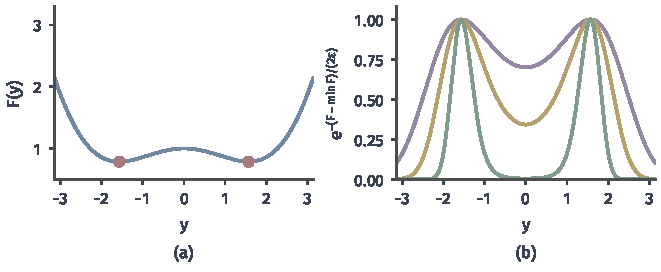
\includegraphics[width=112mm]{figures/06-differential-equations/02-partial-differential-equations/matplotlib/hj-cole-hopf-softmin/figure.pdf}
  \caption{Cole--Hopf公式中的权重，$u_0=\cos y$，$(x,t)=(0,\pi/2)$。(a)$F(y)$，红点是两个极小点。(b)归一化的被积函数，$\varepsilon=0.3$（紫）、$0.1$（黄）、$0.02$（绿）。$\varepsilon$变小时质量集中到极小点。}
  \label{fig:hj-cole-hopf-softmin}
\end{BookInlineFigure}

\begin{theorem}[Cole--Hopf解的极限]
\label{thm:hj-cole-hopf-limit}
设$u_0$有界且$R$-Lipschitz，$H=\lVert\bm{p}\rVert_2^2/2$，$u$是式~\eqref{eq:hj-hopf-lax}。对任意$0<t_1<t_2$，存在常数$C$，使对$t\in[t_1,t_2]$、$\bm{x}\in\mathbb{R}^{d}$和$0<\varepsilon\leq1/2$，
\begin{equation}
  \lvert u_\varepsilon(\bm{x},t)-u(\bm{x},t)\rvert\leq C\varepsilon\ln\frac{1}{\varepsilon}.
  \label{eq:hj-cole-hopf-limit}
\end{equation}
\end{theorem}

\begin{proof}
记$m=\min F=u(\bm{x},t)$，$M=\sup\lvert u_0\rvert$，$\bm{y}^*$为一个极小点。由$F(\bm{x})\leq M$，得$m\leq M$。

先估计积分的上界。由$u_0\geq-M$，得到
\[
  F(\bm{y})\geq-M+\frac{\lVert\bm{x}-\bm{y}\rVert_2^2}{2t}.
\]
取$\rho^2=8Mt$，当$\lVert\bm{x}-\bm{y}\rVert_2\geq\rho$时，
\[
  F(\bm{y})-m\geq\frac{\lVert\bm{x}-\bm{y}\rVert_2^2}{2t}-2M\geq\frac{\lVert\bm{x}-\bm{y}\rVert_2^2}{4t}.
\]
球内用$F\geq m$。合起来，记$\lvert B_\rho\rvert$为半径$\rho$的球的体积，得
\[
  \int\mathrm{e}^{-F/(2\varepsilon)}\,\mathrm{d}\bm{y}\leq\mathrm{e}^{-m/(2\varepsilon)}\bigl(\lvert B_\rho\rvert+(8\pi\varepsilon t)^{d/2}\bigr).
\]

再估计下界。由$\rho$的取法，极小点满足$\lVert\bm{x}-\bm{y}^*\rVert_2\leq\rho$。在$\bm{y}^*$的半径$\varepsilon$的球内，$F$是$\Lambda$-Lipschitz的，$\Lambda=R+(\rho+1)/t$，所以$F\leq m+\Lambda\varepsilon$，积分至少是
\[
  \mathrm{e}^{-m/(2\varepsilon)}\mathrm{e}^{-\Lambda/2}\lvert B_\varepsilon\rvert.
\]

把这两个界代入式~\eqref{eq:hj-cole-hopf}，$-2\varepsilon\ln$作用在$\mathrm{e}^{-m/(2\varepsilon)}$上得到$m$，其余因子是$\varepsilon$的幂次和$t\in[t_1,t_2]$上有界的常数，它们取对数再乘$2\varepsilon$后，不超过$C\varepsilon\ln(1/\varepsilon)$。
\end{proof}

所以在这个模型中，消失黏性的极限就是Hopf--Lax公式，也就是唯一的黏性解。

折角附近的结构也能精确算出。在$(0,\pi/2)$附近，$F$有两个极小点$\pm\pi/2$，$F''(\pm\pi/2)=2/\pi$，也就是$tF''=1$。把积分在两个极小点附近用Gauss积分近似，每个贡献$\sqrt{4\pi\varepsilon/F''}\,\mathrm{e}^{-\pi/(8\varepsilon)}$，于是
\begin{equation}
  u_\varepsilon(0,\pi/2)=\frac{\pi}{4}-2\varepsilon\ln2+O(\varepsilon^2).
  \label{eq:hj-kink-correction}
\end{equation}
其中$\ln2$来自“两个极小点”。表~\ref{tab:hj-kink-correction}用式~\eqref{eq:hj-cole-hopf}的数值积分核对，$\varepsilon$越小吻合得越好。

\begin{BookInlineTable}
  \centering
  \begin{tabular}{cccc}
    \toprule
    $\varepsilon$ & $0.2$ & $0.05$ & $0.01$\\
    \midrule
    $\pi/4-u_\varepsilon(0,\pi/2)$ & $0.2842$ & $0.0800$ & $0.0142$\\
    $2\varepsilon\ln2$ & $0.2773$ & $0.0693$ & $0.0139$\\
    \bottomrule
  \end{tabular}
  \caption{折角处的黏性修正，$u_0=\cos x$，$H=p^2/2$。}
  \label{tab:hj-kink-correction}
\end{BookInlineTable}

两条分支在$x=0$附近可以近似写成$\pi/4\pm x$，软极小给出
\[
  u_\varepsilon\approx\frac{\pi}{4}-2\varepsilon\ln\Bigl(2\cosh\frac{x}{2\varepsilon}\Bigr),\qquad
  \partial_xu_\varepsilon\approx-\tanh\frac{x}{2\varepsilon}.
\]
折角被抹成宽度约$\varepsilon$的过渡层，它的斜率恰好是第~\ref{chap:scalar-conservation-laws}章Burgers方程的黏性激波剖面。图~\ref{fig:hj-viscous-limit}显示这个过程。

\begin{BookInlineFigure}
  \centering
  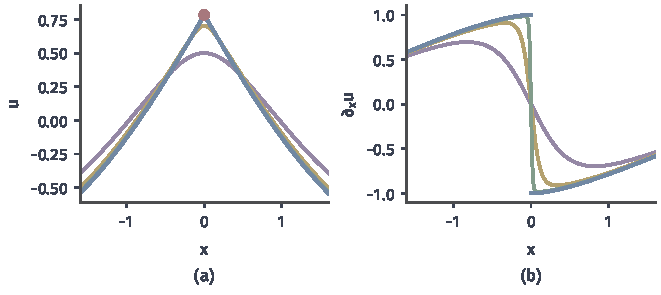
\includegraphics[width=112mm]{figures/06-differential-equations/02-partial-differential-equations/matplotlib/hj-viscous-limit/figure.pdf}
  \caption{消失黏性的极限，$u_0=\cos x$，$t=\pi/2$。(a)式~\eqref{eq:hj-cole-hopf}的$u_\varepsilon$，$\varepsilon=0.2$（紫）、$0.05$（黄）、$0.01$（绿），蓝线是Hopf--Lax解，红点是折角。(b)对应的斜率，$\varepsilon$变小时过渡层变窄，趋向蓝线在$x=0$的跳跃。}
  \label{fig:hj-viscous-limit}
\end{BookInlineFigure}

到达时间也有同样的线性化。令$T_\varepsilon=-\varepsilon\ln w$，代入带小扩散的方程
\[
  \lVert\nabla T_\varepsilon\rVert_2^2-\varepsilon\Delta T_\varepsilon=1,
\]
得到线性方程
\[
  \varepsilon^2\Delta w=w.
\]
第~\ref{chap:pde-problems}章的一维显式解就是$w=\cosh(x/\varepsilon)/\cosh(1/\varepsilon)$。

在平面上，点源的径向解是修正Bessel函数$K_0(r/\varepsilon)$，它满足$\varepsilon^2\Delta w=w$（$r>0$）。两个源的线性叠加给出
\[
  T_\varepsilon=-\varepsilon\ln\Bigl[K_0\bigl(\lVert\bm{x}-\bm{a}\rVert_2/\varepsilon\bigr)+K_0\bigl(\lVert\bm{x}-\bm{b}\rVert_2/\varepsilon\bigr)\Bigr].
\]
$K_0(z)$随$z$增大以$\mathrm{e}^{-z}$的速度衰减，所以$T_\varepsilon$是两个距离的软极小。图~\ref{fig:hj-soft-two-sources}显示，$\varepsilon$变小时，等值线向$T=\min\{T_1,T_2\}$靠拢，中垂线上的尖角由圆滑变尖锐。

\begin{BookInlineFigure}
  \centering
  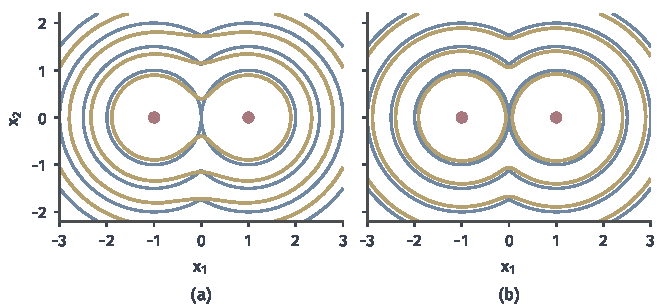
\includegraphics[width=112mm]{figures/06-differential-equations/02-partial-differential-equations/matplotlib/hj-soft-two-sources/figure.pdf}
  \caption{到达时间的软化，源为两个红点。蓝线是$T=\min\{T_1,T_2\}$的等值线$1,1.5,2,2.5$，黄线是$T_\varepsilon$的相同等值线。(a)$\varepsilon=0.3$。(b)$\varepsilon=0.08$。}
  \label{fig:hj-soft-two-sources}
\end{BookInlineFigure}

\paragraph{一般Hamilton量}
一般的$H$没有线性化，但结论不依赖显式解，其根据是黏性解在局部一致极限下稳定。

\begin{theorem}[黏性解的稳定性]
\label{thm:hj-stability-viscosity}
设$H$连续，$u_\varepsilon\in C^2$是式~\eqref{eq:hj-viscous}中方程的经典解，$\varepsilon\to0$时$u_\varepsilon\to u$在$\mathbb{R}^{d}\times(0,t_{\mathrm{f}})$上局部一致成立。则$u$是
\begin{equation}
  \partial_tu+H(\nabla u)=0
  \label{eq:hj-limit-equation}
\end{equation}
的黏性解。
\end{theorem}

\begin{proof}
只证次解，上解同理。设$\varphi\in C^1$，$u-\varphi$在$P$取局部极大。换成$\tilde\varphi=\varphi+\lVert\bm{z}-P\rVert_2^2$（$\bm{z}=(\bm{x},t)$），它在$P$的导数不变，且$u-\tilde\varphi$在$P$取严格局部极大。取以$P$为中心的闭球$B$，$B$在$t>0$内，使$P$是$u-\tilde\varphi$在$B$上唯一的最大点。

取光滑函数$\varphi^\eta$在$B$上连同一阶导数一致收敛到$\tilde\varphi$。固定$\eta$，$u_\varepsilon-\varphi^\eta$在$B$上的最大点记为$P_{\varepsilon}$。当它在$B$的内部时，一阶和二阶条件给出
\[
  \partial_t\varphi^\eta(P_\varepsilon)+H\bigl(\nabla\varphi^\eta(P_\varepsilon)\bigr)=\varepsilon\Delta u_\varepsilon(P_\varepsilon)\leq\varepsilon\Delta\varphi^\eta(P_\varepsilon).
\]

$\varphi^\eta$是固定的光滑函数，$\Delta\varphi^\eta$在$B$上有界。由一致收敛，$\varepsilon\to0$时$P_\varepsilon$的聚点是$u-\varphi^\eta$在$B$上的最大点；$\eta$充分小时这些点都靠近$P$，从而在$B$内部。令$\varepsilon\to0$，得到在某个最大点$P^\eta$处
\[
  \partial_t\varphi^\eta(P^\eta)+H\bigl(\nabla\varphi^\eta(P^\eta)\bigr)\leq0.
\]
再令$\eta\to0$，$P^\eta\to P$，$\varphi^\eta$的导数收敛到$\tilde\varphi$的导数，由$H$的连续性得到$\partial_t\varphi(P)+H(\nabla\varphi(P))\leq0$。
\end{proof}

证明只用到局部一致收敛，这就是黏性解在极限下稳定的原因。不需要梯度的强收敛，而对弱解来说，$H(\nabla u_\varepsilon)$的弱极限一般不是$H(\nabla u)$。

\begin{theorem}[消失黏性选择黏性解]
\label{thm:hj-vanishing-viscosity}
设$H$连续，$u_0$有界且$R$-Lipschitz。设对每个充分小的$\varepsilon$，式~\eqref{eq:hj-viscous}有$C^2$解$u_\varepsilon$，并且存在不依赖$\varepsilon$的常数$C$，使
\begin{equation}
  \lvert u_\varepsilon\rvert\leq C,\qquad\lVert\nabla u_\varepsilon\rVert_2\leq R,\qquad\lvert\partial_tu_\varepsilon\rvert\leq C.
  \label{eq:hj-uniform-estimates}
\end{equation}
则$\varepsilon\to0$时，$u_\varepsilon$局部一致收敛到初值问题唯一的有界、关于$\bm{x}$是$R$-Lipschitz的黏性解。
\end{theorem}

\begin{proof}
由式~\eqref{eq:hj-uniform-estimates}，$\{u_\varepsilon\}$一致有界且等度连续。由Arzel\`a--Ascoli定理，一致有界、等度连续的函数列在紧集上有一致收敛的子列。取任一收敛子列，极限$u$继承相同的界，由定理~\ref{thm:hj-stability-viscosity}是黏性解，$u(\cdot,0)=u_0$。

由定理~\ref{thm:hj-uniqueness}，这样的黏性解只有一个，所以所有收敛子列有相同的极限，整个族收敛。
\end{proof}

式~\eqref{eq:hj-uniform-estimates}是定理的条件，不是自动成立的。对光滑的$H(\bm{p})$，它们来自线性抛物方程的最大值原理：差商$u_\varepsilon(\bm{x}+\bm{h},t)-u_\varepsilon(\bm{x},t)$满足一个线性抛物方程，最大值在初始时刻取得，所以空间Lipschitz常数不增加，时间导数的界要求初值更光滑或先磨光初值。光滑解的存在性证明要用到抛物方程的正则性理论，篇幅较长，可查阅\scite{math-bardi1997hjb}。

所以$\varepsilon\Delta u$的作用和第~\ref{chap:scalar-conservation-laws}章在守恒律中的作用一样：它打破了对称，选择了一个解。$\varepsilon$的符号决定选哪个，这就是第~\ref{chap:pde-problems}章看到的符号问题。

\paragraph{有限黏性的误差}
$\varepsilon>0$时$u_\varepsilon$是光滑的，但它只是近似。一般的Lipschitz初值下，$\sup\lvert u_\varepsilon-u\rvert$的量级是$\sqrt{\varepsilon t}$，证明要用变量倍增并同时估计黏性项，篇幅较长，读者可查阅\scite{math-bardi1997hjb}。这个量级的含义是：在只有Lipschitz正则性时，误差随$\varepsilon$减小得比$\varepsilon$本身慢。在例~\ref{ex:hj-cos}中，由于解的结构特殊，$x=0$处的误差是$O(\varepsilon)$，见式~\eqref{eq:hj-kink-correction}和图~\ref{fig:hj-two-limits}(b)。

\paragraph{不要混淆两个极限}
实际计算时有两个参数：黏性$\varepsilon$和网格步长$h$。令$h\to0$只是更准确地解带$\varepsilon$的方程，令$\varepsilon\to0$才改变方程本身。

图~\ref{fig:hj-two-limits}(a)做了一个实验：固定$\varepsilon=0.1$，用周期网格上的中心差分和显式时间推进，时间步足够小，算到$t=\pi/2$。随着网格加密，到$u_\varepsilon$的误差按$h^2$下降，从$N=20$时的$0.056$降到$N=640$时的$6\times10^{-5}$。到$u$的误差却停在$0.159$附近，这是黏性解与带黏性方程的差，再细的网格也消除不了。

\begin{BookInlineFigure}
  \centering
  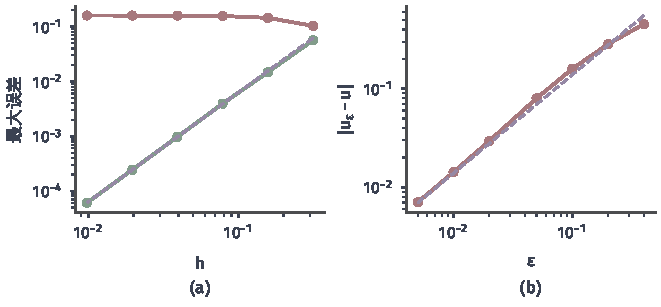
\includegraphics[width=112mm]{figures/06-differential-equations/02-partial-differential-equations/matplotlib/hj-two-limits/figure.pdf}
  \caption{两个极限的区分，$u_0=\cos x$，$t=\pi/2$。(a)固定$\varepsilon=0.1$，网格点数$N=20,\ldots,640$（$h=2\pi/N$），绿线是数值解到$u_\varepsilon$的最大误差，红线是到黏性解$u$的最大误差，紫色虚线是$h^2$的参考斜率。(b)式~\eqref{eq:hj-cole-hopf}在$x=0$处的误差随$\varepsilon$的变化，紫色虚线是$2\varepsilon\ln2$。}
  \label{fig:hj-two-limits}
\end{BookInlineFigure}

要逼近$u$本身，必须同时让$\varepsilon\to0$，并且让网格能够分辨宽度约$\varepsilon$的过渡层，或者在格式里内建适当的数值耗散。后一种做法把$\varepsilon$隐含在网格步长中，两个极限就合并了，这时收敛性需要专门的分析，不能从上面的实验推出。
